
\begin{align}
\because \myvec{\vec{A-C}}^\top\myvec{\vec{B-C}}=\myvec{-1&3&5}\myvec{-2\\1\\-1}\\=0
\end{align}
the triangle in Fig.     \ref{fig:vec/2/4/} is right angled.
\begin{figure}[ht]
    \centering
    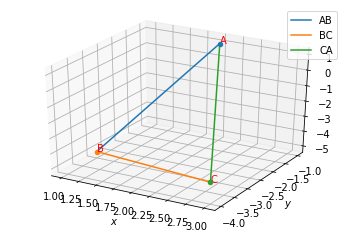
\includegraphics[width=\columnwidth]{solutions/su2021/2/4/Right angle triangle.png}
    \caption{}
    \label{fig:vec/2/4/}
    \end{figure} 

